\label{chap:2}

\section{Contexto Histórico}

    Um problema de biologia relacionado à maneira com que o sistema nervoso central codifica um impulso muscular foi o que levou Hérault, Jutten e Ans a publicarem o trabalho que é considerado a origem da formulação do problema de BSS \cite{french}. O trabalho consistia em tentar obter um modelo computacional que se comportasse como o cérebro humano no momento em que este, a partir de apenas um único sinal nervoso, interpreta duas funções importantes: a translação e a velocidade angular do movimento muscular. Pode-se dizer que este trabalho teve dois principais resultados. O primeiro foi evidenciar a necessidade da aplicação de \textit{HOS} (do inglês, \textit{Higher Order Statistics}) ao problema. Isto foi fundamental na concepção dos métodos para resolução do problema da BSS. O segundo foi a modelagem algébrica dos sistemas de mistura e separação, a matéria-prima do caso BSS/ICA.


    Em 1994, Pierre Comon, utilizando-se dos resultados obtidos por Darmois na década de 1950, formalizou o conceito de ICA e relacionou a independência estatística com o problema da BSS. \cite{Comon}
    
    
    Jean-François Cardoso e Amari obtiveram, de forma independente, um método de otimização frequentemente empregado em BSS, denominado ``\textit{gradiente relativo}" por Cardoso \cite{easi} e ``\textit{gradiente natural}" por Amari \cite{Riemenn}. Cardoso também introduziu os conceitos de maximização por verossimilhança no problema de BSS \cite{ICA3}.
    
    
    O trabalho de Bell e Sejnowski \cite{ICAML} popularizou o problema do BSS na comunidade de processamento de sinais devido à sua simplicade de implementação combinada com a capacidade de separar uma quantidade considerável de fontes.
    
    No fim da década de 1990, os trabalhos de Karhunen, Pajunen e Oja \cite{ICA} possibilitaram analisar a ICA como uma extensão não-linear da técnica PCA, já bastante conhecida e difundida na comunidade. Isto fez com que a ICA pudesse ser aplicada em vários estágios referentes à análise de dados. Além disso,  o trabalho de  Hyvärinen introduz o conceito de maximização da não-gaussianidade \cite{ICAML}, dando origem a um dos algoritmos mais conhecidos para o problema, o FastICA.
    
    
    Atualmente, uma das principais vertentes de estudo do problema de BSS é considerada a dissociação entre BSS e ICA, que pode ser evidenciada por estudos tais como o do algoritmo TRINICON \cite{trinicon}
    
\section{Descrição do Problema}
    
    Consideremos a situação representada na Figura \ref{fig:structure}, onde temos um conjunto de N sinais de fontes submetido à ação de um sistema misturador, isto é, um sistema cujas M saídas correspondem à misturas das suas entradas. O problema de separação cega de fontes reside em recuperar os sinais da entrada deste sistema através apenas das observações dos sinais de saída, ou seja, sem nenhum conhecimento do processo de mistura. Esta é uma peculiaridade da BSS em relação aos outros temas de filtragem, o que a torna particularmente útil em aplicações que são não-supervisionadas. Nestes casos, é inviável ou até mesmo impossível utilizar algum sinal no canal para tentar ajustar o sistema separador. Dessa falta de informação sobre o processo de mistura é que provem a nomenclatura \textit{cega}.
    
    \begin{figure}
       \hfill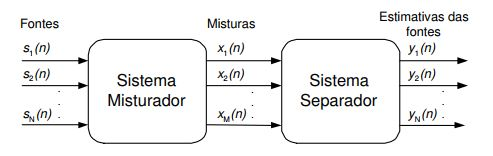
\includegraphics[scale=1.0]{fig221.JPG}\hspace*{\fill}
        \caption{Estrutura do problema de Separação Cega de Fontes.}
        \label{fig:structure}
    \end{figure}


\section{Aplicabilidade}
    Devido à generalidade do problema de BSS, várias aplicações podem se beneficiar dos métodos desenvolvidos para encontrar as melhores soluções. Veremos, nesta seção, algumas aplicações de destaque das técnicas de BSS nas diferentes áreas.
    
\subsection{Biomedicina}
    Na biomedicina, a busca por métodos não-invasivos que ainda se mostrem confiáveis é um desafio. O EEG (Eletroencefalograma) e o ECG (Eletrocardiograma) são dois exemplos bem comuns de técnicas que satisfazem esta necessidade. Entretanto, é relativamente difícil captar apenas os sinais desejados quando os sensores são posicionados em uma determinada região do corpo humano, principalmente devido à interferência proveniente de sinais gerados por outras atividades fisiológicas.
       
    Uma forma de resolver este problema está na repetição da realização do exame, o que pode não ser viável em certas ocasiões, além de causar fadiga nos pacientes. O emprego de técnicas de BSS oferece uma alternativa eficiente, uma vez que o processamento é dado após a coleta dos dados e requer apenas um experimento.
    
    Existe uma expressiva gama de trabalhos acerca de separação de sinais biomédicos, o que evidencia sua importância.
    
\subsection{Telecomunicações}

    A BSS está diretamente ligada a um tema relevante em telecomunicações: a equalização de canais. A idéia essencial de um sistema de comunicação é fazer com que a informação enviada por um transmissor possa ser obtida de maneira tão fiel ao original quanto possível por um receptor. Assim sendo, mitigar distorções introduzidas pelo canal é fundamental. Em outra estratégia, a equalização do canal, utiliza-se um filtro (equalizador) no receptor de modo que este seja capaz de reduzir significativamente os efeitos do canal. Em essência, o desenvolvimento de técnicas de equalização está intimamente relacionado à concepção de critérios que guiem o ajuste dos parâmetros livres do equalizador de modo que se obtenha uma boa estimativa do sinal transmitido.
    Por exemplo, em um dos paradigmas mais conhecidos, adota-se como critério a minimização do erro quadrático médio entre a saída do equalizador e o sinal desejado, no caso, o sinal transmitido \cite{Haykin}. Os critérios presentes na equalização não-supervisionada (ou cega) utilizam, além dos sinais recebidos, apenas algumas informações estatísticas dos sinais transmitidos. Uma vantagem desta estratégia em relação ao paradigma supervisionado é a possibilidade de realizar o ajuste dos parâmetros concomitantemente com a transmissão dos dados.
    
\subsection{Separação de sinais de áudio}

    Imagine a seguinte situação: uma pessoa se encontra em uma sala onde existem diversos grupos de pessoas conversando concomitantemente, como, por exemplo, em uma reunião. Além disso, há ruído de fundo gerado, por exemplo, por música ambiente e ecos no recinto. Apesar de todas essas interferências, o ser humano é capaz de distinguir a voz ou o som de interesse em um determinado momento. Essa habilidade é conhecida na literatura como \textit{cocktail-party effect}\cite{cocktail}, justamente pela analogia com o cenário descrito.

    Este caso levou ao questionamento: será possível a um sistema de processamento artificial alimentado apenas por gravações de microfones posicionados pela sala distinguir o sinal de voz de uma pessoa qualquer? Ao passo que o cérebro humano resolve com certa facilidade este problema, o desenvolvimento de sistemas automáticos para realizar tal tarefa ainda corresponde a um complexo desafio.

\section{Modelagem Matemática do Problema}\label{sec:model}
    Neste capítulo, iremos descrever como o problema de BSS pode ser resolvido. Primeiramente, é necessário buscar modelos matemáticos capazes de expressar o comportamento do sistema em função do misturador e do separador.
    
    Considere que cada elemento do vetor $\mathbf{s}$($\mathpzc{n}$) = [${s_1}$($\mathpzc{n}$) ${s_2}$($\mathpzc{n}$) \dots  $s_N$($\mathpzc{n}$)]$^T$ corresponde a um sinal da fonte emissora. Analogamente, representamos os sinais misturados pelo vetor  $\mathbf{x}$($\mathpzc{n}$) = [${x_1}$($\mathpzc{n}$) ${x_2}$($\mathpzc{n}$) \dots  ${x_M}$($\mathpzc{n}$)]$^T$. De forma generalizada, o sistema misturador pode ser representado pela expressão:

    \begin{equation}\label{eq:mixer}
        \mathbf{x}(\mathpzc{n}) = \mathcal{F}(\mathbf{s}(\mathpzc{n}), \mathbf{s}(\mathpzc{n-1}), \dots, \mathbf{s}(\mathpzc{n - L}), \mathbf{v}(\mathpzc{n})),
    \end{equation}
    onde o operador $\mathcal{F}$($\cdot$) descreve a ação do sistema misturador, $L$ corresponde ao número de amostras passadas (memória) do vetor de fontes e o vetor $\mathbf{v}$($\mathpzc{n}$) corresponde ao ruído associado às fontes ou sensores do sistema.
    
    Vale ressaltar que a representação \ref{eq:mixer} tem caráter puramente didático, uma vez que não existem técnicas de BSS que lidem com todos estes efeitos representados e uma só vez. Em geral, as técnicas são aplicadas a casos específicos, isto é, versões simplificadas da formulação citada. Desta forma, torna-se necessário introduzir os conceitos de classificação de um sistema misturador para auxiliar na adequação do problema para o caso proposto por este trabalho.
    
    \textbf{Sistemas Lineares e Não-Lineares} O sistema misturador é dito linear se o operador  $\mathcal{F}$($\cdot$) respeita o princípio da superposição, conforme descrito abaixo:

        % Linearidade
        \begin{equation}\label{eq:linearity}
            \mathcal{F}(\mathbf{a_1}\mathbf{s_1}(\mathpzc{n}) + \mathbf{a_2}\mathbf{s_2}(\mathpzc{n})) = \mathpzc{a_1}\mathcal{F}(\mathbf{s_1}(\mathpzc{n})) + \mathpzc{a_2}\mathcal{F}(\mathbf{s_2}(\mathpzc{n}))
        \end{equation}
    para quaisquer constantes $\mathpzc{a_1}$ e $\mathpzc{a_2}$ e vetores $\mathbf{s_1}$ e $\mathbf{s_2}$. Caso contrário, o sistema é classificado como não-linear. 
    
     \textbf{Sistemas Instântaneos e Convolutivos} Nos casos em que o sistema depende de amostras passadas, isto é, $L>0$, o sistema é dito convolutivo. No caso em que $L=0$, o sistema é dito instantâneo.
    
     \textbf{Sistemas Sub-Determinados, Determinados e Sobre-Determinados} Quando o número de sensores é maior que o número de fontes ($M>N$), tem-se o caso sobre-determinado. Analogamente, o caso sub-determinado corresponde ao caso em que $M<N$. O caso em que $M=N$ é chamado de determinado.
     
     Apesar da característica principal da BSS ser a falta de informação sobre o processo de mistura, é fundamental ao menos ter-se um certo conhecimento sobre a estrutura do sistema misturador. Assim, é possível definir um separador estruturalmente capaz de reverter a ação do processo de mistura. Geralmente, este tipo de informação é obtido com base na aplicação de interesse. No caso deste trabalho, o problema de separação de sinais de áudio, o processo de mistura é geralmente convolutivo, devido à presença de reverberações no ambiente.
     
     A maioria dos trabalhos acerca de BSS abordam cenários com sistemas misturadores lineares e com o mesmo número de fontes e sensores, diferenciando-se basicamente no contexto de misturas instantâneas ou convolutivas. Apesar desta última classificaçãço desempenhar um papel fundamental na abordagem do problema, o  processo de mistura pode ser igualmente descrito matematicamente da seguinte forma:
     
     % Notação Matricial
     \begin{equation}\label{eq:xn}
        \mathbf{x} = \mathbf{A}\mathbf{s},
    \end{equation}
    onde a matriz $\mathbf{A}$ de dimensão ${N \times N}$ é chamada de matriz de mistura. A diferença é que, no caso linear, os elementos da matriz $\mathbf{A}$ são constantes que multiplicam as componentes do vetor de fontes $\mathbf{s}$ para formar as misturas $\mathbf{x}$, enquanto no caso convolutivo, os elementos da matriz $\mathbf{A}$ são, geralmente, filtros \textit{FIR} que representam o percurso realizado pela fonte até o sensor, devido à presença de reverberação. Assim, tem-se a convolução de cada uma das respostas ao impulso desses filtros com cada elemento do vetor de fontes $\mathbf{s}$. A despeito de sua simplicidade, esta classe de modelos é válida em uma vasta quantidade de problemas de BSS \cite{ICA}. Além disso, é possível recuperar as fontes através da Análise de Componentes Independentes, que será visto na próxima seção.

\section{Análise de Componentes Independentes} \label{sec:ICA}
    Nesta seção serão apresentados os aspectos básicos da ICA (do inglês, \textit{Independent Component Analysis}), relacionando-a com alguns métodos semelhantes. Embora a ICA seja definida para o caso linear e convolutivo, trataremos apenas do caso linear, pois é o que condiz com a abordagem que queremos realizar, a de separação das fontes no domínio da frequência. Recomendamos ao leitor interessado em um estudo aprofundado sobre os aspectos teóricos da ICA a leitura do trabalho de Comon \cite{Comon}, responsável pela formalização matemática desse assunto, e as referências  \cite{ICA3}, \cite{ICA}.
    
    Os algoritmos ICA podem ser derivados através da estimativa da máxima verossimilhança \cite{ICAML}, \cite{ML}, \cite{NaturalICA} e da maximização da não-gaussianidade \cite{fastica1}, \cite{fastica2}, \cite{fastica3} e \cite{fasticaebm}. Apesar da maioria dos algoritmos serem desenvolvidos para trabalhar com números reais, podemos estende-los para lidar com números complexos. Para isto, é preciso escolher apropriadamente uma função não-linear \textit{G} que, relacionada à formulação dos algoritmos para sinais reais, permita o emprego dos mesmos para sinais complexos.

\subsection{Definição}
    Devido à sua natureza recente, não é difícil encontrar ao menos duas definições distintas para a ICA na literatura. Entretanto, utilizaremos a definição que mais se aproxima com a aplicação que é o objetivo deste trabalho.
    
    \medskip
    
    \textbf{Definição 2.5.1 (ICA)} A ICA de um vetor aleatório $\mathbf{x}$ = [${x_1}$ ${x_2}$ $\dots$  ${x_M}]^T$ consiste em determinar o segundo modelo generativo linear (ou modelo ICA):
    
    \begin{equation}\label{eq:simplifiedmixer}
        % Notação Matricial
        \mathbf{x} = \mathbf{A}\mathbf{s},
    \end{equation}
    onde os elementos de $\mathbf{s}$ = [${s_1}$ ${s_2}$ \dots  ${s_N}$]$^T$ são estatisticamente independentes entre si e $\mathbf{A}$ corresponde a uma matriz constante de dimensão $M\times N$.
    \bigskip 
    
    Sob a hipótese de que os sinais fontes são estatisticamente independentes entre si, fica claro que os elementos de $\mathbf{x}$ não são mais independentes, devido ao processo de mistura. O ponto fundamental da aplicação da ICA diz respeito exatamente a esta constatação, no sentido de que essa metodologia se propõe a separar as fontes a partir da recuperação da independência. O sistema separador, implementado pela matriz $\mathbf{W}$, é ajustado de modo que as compomentes do vetor $\mathbf{y}$ de estimativas das fontes sejam as mais independentes possíveis entre si.
    
    Entretanto, esta abordagem levanta a seguinte questão: tornar as estimativas das fontes independentes implica necessariamente na recuperação das fontes? Foi Pierre Comon \cite{Comon} que não só respondeu a esta pergunta, mas também forneceu todo o respaldo matemático necessário para o desenvolvimento da ICA e, por consequência, da BSS.
    A partir do teorema de Darmois, ele mostrou que é possível separar as fontes com base na recuperação da independência estatística, respeitando algumas condições para as fontes e para o sistema separador.

\subsection{Separabilidade}\label{sec:separability}

    O modelo descrito na Seção \ref{sec:model} é dito separável se, para toda matriz separadora $\mathbf{W}$ que resulte em um vetor $\mathbf{y}$ que tem os elementos estatísticamente independentes entre sim, tem-se que $\mathbf{y}$ = $\mathbf{Wx}$ = $\mathbf{\Lambda P s}$, onde $\mathbf{\Lambda}$ e $\mathbf{P}$ representam matrizes diagonal e de permutação, respectivamente. Assim, em um modelo separável, é possível obter as fontes através da ICA. Entretanto, é importante ressaltar que surgem duas ambiguidades associadas a este modelo: A ordem das fontes e seus ganhos de escala. Mediante este problema, Comon \cite{Common} formulou o seguinte teorema, evidenciando as condições necessárias para que um sistema misturador linear seja separável:
    
    \bigskip
    
    \textbf{Teorema 2.5.1 (Separabilidade)} O modelo $\mathbf{x} = \mathbf{As}$ é separável se e somente se a matriz $\mathbf{A}$ possuir posto completo e, no máximo, um dos elementos do vetor $\mathbf{s}$ for gaussiano.
    
    \bigskip
    
    Este teorema inclui mais uma restrição à aplicação da ICA, que é a incapacidade de recuperar fontes gaussianas. Na próxima seção, trataremos da utilização de estatísticas de segunda ordem para realizar a separação e este problema será melhor ilustrado. Também discutiremos porque a utilização da correlação, uma medida mais ``fraca", não é capaz de resolver o problema, mas pode ser bastante útil numa etapa de pré-processamento.
  
\subsection{Técnicas baseadas em estatístiscas de segunda ordem aplicadas à BSS}\label{secondorder}

    Até a década de 1980, a maioria das técnicas de filtragem estatística eram baseadas em estatísticas de segunda ordem. Isto era devido à simplicadade matemática relacionada a este tipo de abordagem e ao fato de que modelos gaussianos de sinais eram praticamente os únicos utilizados. 
    
    Foi durante o desenvolvimento da teoria de filtragem não-supervisionada, dentro do contexto de identificação e equalização cega, que se chegou à conclusão de que, para resolver essa classe de problemas, era necessário utilizar \textit{HOS} \cite{HOS}. Em BSS, esse conhecimento é fundamental.
    
    Na seção anterior mostramos que o problema da BSS pode ser resolvido com base na independência estatística, isto é, através de \textit{HOS}, uma vez que a independência requer conhecimento da densidade de probabilidade e, por consequência, todas as estatísticas de uma variável aleatória. Entretanto, esta seção será voltada para a apresentação da abordagem utilizando apenas estatísticas de segunda ordem para BSS, mostrando que isto não é suficiente para a resolução do problema.
    
    \subsubsection{Descorrelação}
    Com base no modelo ICA apresentado na Seção \ref{sec:model}, obtemos a matriz de correlação entre as misturas, dada por:
    \begin{equation}
        \label{eq:correlationmatrixforx}
        \begin{split}
        \mathbf{R_x} & = \mathpzc{E}\{\mathbf{xx^T}\}\\
                     & = \mathpzc{E}\{\mathbf{(As)(As)^T}\}\\
                     & = \mathpzc{E}\{\mathbf{Ass^TA^T}\} \\
                     & = \mathbf{A}\mathpzc{E}\{\mathbf{ss^T}\}\mathbf{A^T} \\
                     & = \mathbf{A}\mathbf{R_s}\mathbf{A^T} \\
                     & = \mathbf{A}\mathbf{A^T}, \\
        \end{split}
    \end{equation}
    onde $\mathbf{R_s}$ corresponde à matriz de correlação do vetor das fontes. Como estamos utilizado a hipótese de que as fontes são estatísticamente independentes e possuem variância unitária, esta matriz é igual à identidade.
    
    Após passar por um sistema separador, a correlação entre as estimativas das fontes é descrita por:
    \begin{equation}
        \label{eq:correlationmatrixfory}
        \begin{split}
        \mathbf{R_y} & = \mathpzc{E}\{\mathbf{yy^T}\}\\
                     & = \mathpzc{E}\{\mathbf{(Wx)(Wx)^T}\}\\
                     & = \mathpzc{E}\{\mathbf{Wxx^TW^T}\} \\
                     & = \mathbf{W}\mathpzc{E}\{\mathbf{xx^T}\}\mathbf{W^T} \\
                     & = \mathbf{W}\mathbf{R_x}\mathbf{W^T}\\
        \end{split}
    \end{equation}
    
    Assim, para descorrelacionarmos as saídas do sistema separador, precisamos determinar $\mathbf{W}$ tal que $\mathbf{R_y = I}$. Solucionando a equação, chegamos à conclusão de que:
    
    \begin{equation}
        \label{separationmatrixsolution}
        \mathbf{W} = \mathbf{D}^{-\frac{1}{2}}\mathbf{E^T}
    \end{equation}
    
    Entretanto, se consideramos o caso em que o sistema separador é dado pela expressão $\mathbf{QW}$, onde $\mathbf{Q}$ corresponde a uma matriz ortogonal (i.e., sua inversa coincide com sua transposta). Substituindo na solução da equação (\ref{eq:correlationmatrixfory}), fica claro ver que o resultado permanece o mesmo. Isto mostra que a recuperação das fontes utilizando apenas a informação da descorrelação apresenta uma indeterminação relacionada a um fator ortogonal.
    
    A seguir, ilustramos geometricamente o problema. Com este objetivo, exibimos as Figuras \ref{fig:first_sub}, \ref{fig:second_sub} e \ref{fig:third_sub} as distribuições conjuntas de duas fontes, as misturas e suas estimativas obtidas pelo processo de branqueamento, respectivamente. Como o sistema misturador linear é modelado por uma matriz, as misturas são geradas a partir de rotações e escalonamentos das fontes. Apesar do braqueamento conseguir recuperar as escalas das fontes, ele não consegue recuperar a rotação devido à indeterminação referente a uma matriz ortogonal, cujo efeito é a rotação dos dados.
    
    Esta ineficácia na recuperação de fontes gaussianas mostra a limitação da estatística de segunda ordem. Entretanto, a aplicação do branqueamento como um pré-processamento pode ajudar bastante no processo de separação, visto que este faz aproximadamente metade do trabalho de separação.
    
\begin{figure}
    \centering
    \subfigure[Distribuição conjunta das fontes.]
    {
        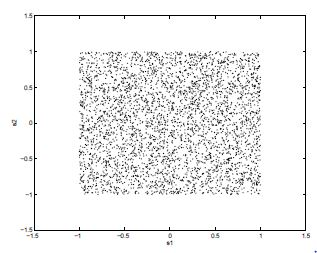
\includegraphics[scale=0.8]{distrib_fontes.JPG}
        \label{fig:first_sub}
    }
    \subfigure[Distribuição conjunta das misturas.]
    {
        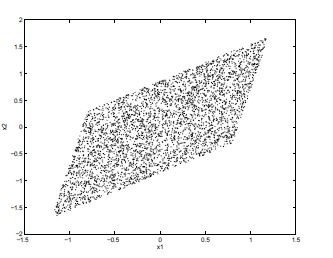
\includegraphics[scale=0.8]{distrib_misturas.JPG}
        \label{fig:second_sub}
    }
    \\
    \subfigure[Distribuição conjunta das estimativas.]
    {
        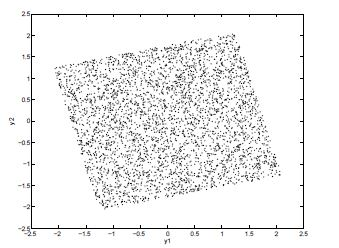
\includegraphics[scale=0.8]{distrib_estimat.JPG}
        \label{fig:third_sub}
    }
    \caption{Tratamento da BSS considerando estatística de segunda ordem.}
    \label{fig:sample_subfigures}
\end{figure}


\subsection{Modelo de maximização da não-gaussianidade}
    
    Um dos principais atrativos presentes nessa estratégia é a possibilidade de recuperar cada uma das fontes individualmente. Um dos algoritmos mais conhecidos em BSS, o FastICA \cite{fastica1}, se baseia neste critério. Para entendermos a abordagem via maximização da não-gaussianidade, precisamos introduzir o conceito de medição da independência entre duas estimativas de fontes, observando sua não-gaussianidade.Para issso, utiliza-se o Teorema Central do Limite \cite{cetrallimit}
    
    \medskip
    
    \textbf{Teorema 2.5.2 (Teorema Central do Limite)} Dadas ${n}$ variáveis aleatórias independentes $\mathpzc{x_i}$, formamos sua soma $\mathpzc{x = x_1 + \dots + x_n.}$. Esta é uma variável aleatória com média $\mathpzc{\eta = \eta_1 + \dots + \eta_n}$ e variância $\mathpzc{\sigma^2 = \sigma_1^2 + \dots + \sigma_n^2}$. O Teorema Central do Limite diz que, dentro de certas condições gerais, a distribuição ${F(x)}$ de $\mathpzc{x}$  se aproxima de uma distribuição normal com a mesma média e variância à medida que ${n}$ cresce.
    
    \medskip
    
    Em termos práticos, quanto mais fontes compuserem uma mistura, mais gaussiana ela será. Existem duas formas de medir a gaussianidade: a curtose e a negentropia.

\subsubsection{Curtose}
    
    A curtose é uma estatística de quarta ordem que categoriza as distribuições como gaussiana, subgaussiana e super-gaussiana. Também pode ser interpretada como o grau de desvio da inclinação em relação à curva de uma distribuição gaussiana e é definida como
    
    \begin{equation}
        \mathpzc{k_4} = \mathpzc{E}\{\mathpzc{x^4}\} - 3(\mathpzc{E}\{\mathpzc{x^2}\})^2.
    \end{equation} 
    
    A curtose é não-nula para a grande maioria das variáveis aleatórias, salvo os sinais gaussianos. Assim, podemos estender o conceito de maximização da não-gaussianidade para a maximização do valor absoluto da curtose do conjunto das fontes. Essa abordagem foi proposta em \cite{ML}, juntamente à deflação, que tem por objetivo a extração das fontes de maneira sequencial.
    
    Segundo o autor em \cite{LuizVictorio}, a derivação do algoritmo de maximização da curtose resulta em:
    \begin{equation}
        \mathbf{w_i} \leftarrow \mathbf{w_i} + \eta  sign(curt_{ICA}(\mathbf{w_iz}))\mathpzac{E}\{\mathbf{z^T}(\mathbf{w_iz})^3\}
        \label{eq:refreshforcurtosis}
    \end{equation}
    \begin{equation}
        \mathbf{w_i} \leftarrow \frac{\mathbf{w_i}}{|| \mathbf{w_i}||},
    \end{equation}
    onde o termo $curt_{ICA}$ tem a seguinte definição:
    \begin{equation}
        curt_{ICA} = \mathpzc{E}\{(\mathpzc(y - \mu_y)^4\} -3\sigma_y^4
    \end{equation}

    Existem basicamente duas abordagens para este caso: a baseada em um gradiente (que faz com que o mesmo necessite uma sábia escolha de um passo de adaptação, podendo resultar em convergência lenta ou até mesmo divergência) e a de ponto fixo, que é a base do FastICA \cite{fastica1}. 
    
    Sobre a abordagem de ponto fixo, seja $\mathpzc{f}$ uma função definida para todos os números reais. A partir de um ponto inicial $\mathpzc{x_0}$, a regra de iteração para o ponto fixo se dá através de 
    \begin{equation}
        \mathpzc{x_{n+1}} = \mathpzc{f(x_n)}, \mathpzc{n = 0,1,2,}\dots,
    \end{equation}
    gerando uma sequência que converge para um ponto fixo da função dado por
    \begin{equation}
        \mathpzc{f(x_{FP})} = \mathpzc{x_{FP}}.
    \end{equation}
    Para que este algoritmo convirja para este ponto estável, o gradiente deve apontar na direção de $\mathbf{w_i}$. Somente assim, quando adicionarmos o gradiente a $\mathbf{w_i}$ em (\ref{eq:refreshforcurtosis}), o vetor $\mathbf{w_i}$ manterá a sua direção, apesar de sua norma $\mathbf{||w_i||}$ se modificar. A abordagem do FastICA propõe algumas simplificações \cite{fastica1}, chegando ao algoritmo na sua forma final:
    
    \begin{equation}
        \mathbf{w_i} \leftarrow \mathpzac{E}\{\mathbf{z^T}(\mathbf{w_iz})^3\} - 3\mathbf{w_i}
        \label{eq:ICAcurtosis}
    \end{equation}
     \begin{equation}
        \mathbf{w_i} \leftarrow \frac{\mathbf{w_i}}{||\mathbf{w_i}||}
        \label{eq:ICAcurtosismodulate}
    \end{equation}

    \bigskip

    Entretanto, o problema com \textit{outliers}, que correspondem às observações da amostra que desviam completamente das demais, tem bastante influência na pouca utilização do método, uma vez que um \textit{outlier} pode mudar completamente a curtose. Por conta disto, neste trabalho não serão abordados algoritmos que utilizem este conceito.
    
\subsubsection{Negentropia} \label{sec:negentropy}

    Já a abordagem da negentropia é mais robusta, apesar de ser computacionalmente mais intensa. Entretanto, existem aproximações simples que garantem um resultado satisfatório nesta abordagem. A entropia é um conceito da Teoria da Informação e está relacionada à incerteza associada à uma variável aleatória. Quanto maior o seu valor, mais aleatória é a variável. Um resultado fundamental da Teoria da Informação é de que uma variável contínua com distribuição gaussiana tem a maior entropia diferencial entre todas as variáveis de igual variância \cite{entropy}. Assim, uma forma de maximizar a não-gaussianidade seria minimizar as entropias marginais das estimativas das fontes. Um problema da entropia diferencial é que seu valor é alterado quando a variável aleatória é multiplicada por uma constante. Para resolver este problema, introduzimos o conceito de negentropia, que é uma normalização da entropia de forma que fique invariante à qualquer transformação linear invertível. A negentropia de uma variável aleatória $\mathpzc{x}$ é dada por:
    \begin{equation}
        \mathpzc{J(x) = H(x_g) - H(x)},
    \end{equation}
    onde $\mathpzc{x_g}$ representa uma variável aleatória gaussiana com a mesma variância de $\mathpzc{x}$. Desta forma, a negentropia é sempre não-negativa e só é igual à zero quando $\mathpzc{x}$ for uma variável gaussiana. Uma vantagem da negentropia é que esta medida de gaussianidade é consideravelmente mais robusta a \textit{outliers} se comparada à curtose.
    Entretanto, há uma dificuldade em relação à sua aplicação devido à necessidade de estimação da entropia. Para tentar contornar isto, é comum escolher uma função não-linear não-quadrática $G(\cdot)$ e incorpora-la à formulação tradicional do método \cite{fastica1}, dada por:
    \begin{equation}
        \mathpzc{J(y)} = \alpha(\mathpzc{E}\{\mathpzc{G(y)}\} - \mathpzc{E}\{\mathpzc{G(\nu)}\})^2,
    \end{equation}
    onde $\alpha$ é uma constante e $\nu$ é uma variável aleatória gaussiana de média zero e variância unitária.  O algoritmo de adaptação da matriz separadora usando maximização da negentropia é dado por:
    \begin{equation}
          \mathbf{w_i} \leftarrow  \mathbf{w_i} + \eta[\mathpzc{E}\{\mathpzc{G(\nu)}\} - \mathpzc{E}\{\mathpzc{G}\mathbf{w_iz}\}]\mathpzc{E}\{\mathbf{z^Tg(w_iz)}\}
    \end{equation}
    \begin{equation}
          \mathbf{w_i} \leftarrow  \frac{\mathbf{w_i}}{||\mathbf{w_i}||},
    \end{equation}
    onde $\mathpzc{g} = \mathpzc{G}'$ é a primeira derivada da função não-quadratíca $\mathpzc{G}$.
    Assim como o caso da curtose, também é possível derivar o algoritmo de ponto fixo para este caso. Conforme descrito em \cite{LuizVictorio}, encontra-se o seguinte algoritmo:
    
    \begin{equation}
        \mathbf{W} \leftarrow \mathpzc{E}\{\mathpzc{g}\mathbf{(y)z^T}\} - diag(\mathpzc{E}\{\mathpzc{g'}\mathbf{(y)}\}\mathbf{W}
    \end{equation}
    
    \begin{equation}
        \mathbf{W} \leftarrow (\mathbf{WW^T})^{-\frac{1}{2}}\mathbf{W}
    \end{equation}
    
    
    Assim sendo, resta escolhar uma função \textit{G} que contenha boas propriedades de convergência ao mesmo tempo que seja uma boa aproximação da entropia. A função $G(s_i)$ = -log($q(s_i)$), onde $q(s_i)$ é a densidade de probabilidade estimada da fonte $s_i$ é uma escolha natural. O problema se torna estimar as densidades de probabilidade das fontes, mas na Figura \ref{fig:scoretable} exibimos as densidades de probabilidade em conjunto com as chamadas funções $g$, também chamadas de funções \textit{score}.
    
    \begin{figure}
        \centering
        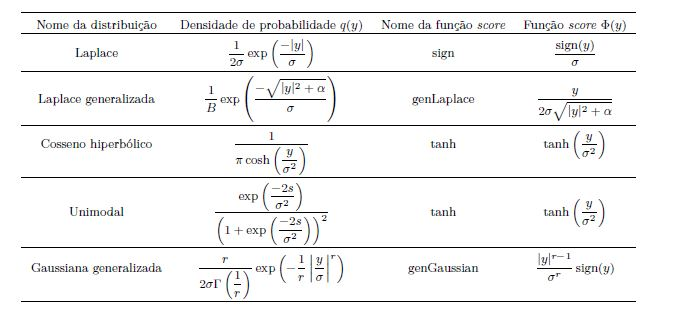
\includegraphics[scale=0.7]{table.JPG}
        \caption{Funções score para diferentes densidades de probabilidade de fontes reais.}
        \label{fig:scoretable}
    \end{figure}
    
\subsection{Modelo de estimação por máxima verossimilhança}

    A maioria dos critérios utilizados pelo caso linear da BSS, embora tenha ligações com o ICA, surgiram a partir de outras idéias que não necessariamente estão ligadas à independência estatística. O caso da estimação por máxima verossimilhança é um dos exemplos mais consagrados deste grupo. Apresentaremos, nesta seção, seus conceitos e como a mesma se relaciona com o problema de BSS. 
    O objetivo por trás da ML (do inglês, \textit{Maximum Likelihood}) é determinar um conjunto de parâmetros $\mathbf{\theta} = [\theta_1, \dots, \theta_n]$ a partir de um conjunto de amostras $\mathbf{e} = [e(1), \dots, e(P)]$ que contém informações sobre eles. As estimativas de $\mathbf{\theta}$ são denotadas por $\hat{\theta}$ e determinadas através da maximização da chamada função de máxima verossimilhança $\mathbf{L(\theta)}$, conforme    
    \begin{equation}\label{eq:argmax}
    \hat{\theta} = \operatorname*{arg\,max}_{\theta} \mathbf{L(\theta)}
    = \operatorname*{arg\,max}_{\theta}
    \mathpzc{p_e}(\mathbf{e} | \mathbf{\theta})
    \end{equation} ou seja, a abordagem por máxima verossimilhança busca o conjunto de parâmetros que maximiza a probabilidade condicional de $\mathbf{e}$ dado $\mathbf{\theta}$.
    
    É comum assumir a independência estatística entre as amostras de $\mathbf{e}$. Assim sendo, podemos reescrever a função de máxima verossimilhança como
    
    \begin{equation}\label{eq:argmax2}
        \mathbf{L(\theta)}
        =\mathpzc{p_e}(\mathbf{e} | \mathbf{\theta})
        =\prod_{p=1}^P \mathpzc{p_e}(\mathbf{e}(\mathpzc{p}) | \mathbf{\theta})
    \end{equation}

    Com relação ao emprego da estimação por máxima verossimilhança no problema de BSS, os parâmetros a serem determinados são os elementos elementos da matriz de mistura $\mathbf{A}$ e os dados disponíveis são as amostras do vetor de misturas $\mathbf{x}$. Assim, segundo \cite{cetrallimit} e considerando a hipótese de independência entre as fontes, temos:
        \begin{equation}\label{eq:verobss}
          \begin{split}
         \mathbf{L(A)} & =\prod_{p=1}^P \mathpzc{p_x}(\mathbf{x}(\mathpzc{p}) | \mathbf{A})\\
                                & =\prod_{p=1}^P\frac{\prod_{n=1}^N\mathpzc{p_{s_n}}(\mathbf{\tilde{a_n}}\mathbf{x}(\mathpzc{p}))}{| det(\mathbf{A}) |},
        \end{split}
    \end{equation} 
    onde termo $\mathbf{\tilde{a}_n}$ corresponde a $\mathpzc{n}$-ésima linha da matriz inversa de $\mathbf{A}$. Também é possível descrever a função de máxima verossimilhança em termos da matriz separadora $\mathbf{W}$, dada por:
    \begin{equation}
        \label{eq:veroForW}
        \mathbf{L(W)} = \prod_{p=1}^{P}\prod_{i=1}^N\mathpzc{p_{s_n}}(\mathbf{w_nx}(\mathpzc{p}))|\text{det}(\mathbf{W})|
    \end{equation}
  
    Entretanto, é comum utilizar-se do logaritmo da verossimilhança, uma vez que é algebricamente mais simples e o máximo ainda é encontrado no mesmo ponto. Assim sendo, obtemos a equação
    
        \begin{equation}
        \label{eq:logverossimilance}
        log(\mathbf{L(W)}) = \mathpzc{E}\{\sum_{i=1}^Nlog(\mathpzc{p_{s_n}}(\mathbf{w_nx}(\mathpzc{p})) + \text{P log}(|det(\mathbf{W})|)\}
    \end{equation}
    
    onde o operador $\mathpzc{E}\{\cdot\}$ representa a estimativa do valor esperado. O valor máximo da verossimilhança pode ser encontrado iterativamente, utilizando-se o gradiente estocástico da verossimilhança. Dois dos principais algoritmos que utilizam a estimativa da ML são o Natural ICA \cite{NaturalICA} e o algoritmo Bell-Sejnowski \cite{ICAML}.
    
    O algoritmo Bell-Sejnowski converge muito lentamente, devido à inversão da matriz separadora $\mathbf{W}$. Este é um caso onde o processo de branqueamento, apresentado na Seção \ref{sec:separability}, e que será visto novamente à frente, ajuda bastante na convergência. Entretanto, o Natural ICA possui uma convergência melhor sem precisar necessariamente de um pré-processamento, tornando o algoritmo Bell-Sejnowski obsoleto.
    
    O gradiente, segundo a definição matemática tradicional, aponta para a direção de maior inclinação em um espaço Euclidiano. Porém, o espaço de busca de parâmetros no ICA não é sempre Euclidiano, mas tem uma estrutura métrica Riemaniana \cite{Riemenn}. Neste caso, deve ser utilizado o chamado gradiente natural, que aplicado à verossimilhança em (\ref{eq:veroForW}), dá origem ao algoritmo Natural ICA.
    
    Definindo-se por $\mathcal{J}$ a função objetivo em função do parâmetro $\mathbf{W}$, temos que o gradiente usual e o gradiente natural são dados, respectivamente, por
    
    \begin{equation}
        \label{eq:gradiente}
        \nabla\mathpzc{J} = \frac{\partial \mathpzc{J}(\mathbf{W})}{\partial \mathbf{W}}
    \end{equation}
    \begin{equation}
        \label{eq:naturalgradiente}
        \nabla\mathpzc{J} = \frac{\partial \mathpzc{J}(\mathbf{W})}{\partial \mathbf{W}}\mathbf{W^T}\mathbf{W}
    \end{equation}
    onde a diferença reside na inclusão do produto com o termo quadrático de $\mathbf{W}$ para o caso do Natural ICA.
    
    A atualização da matriz separadora $\mathbf{W}$ é dada em (\ref{eq:refresh}). Esta equação depende apenas das amostras $\mathbf{y}$ e não possui nenhuma restrição. Isto torna essa abordagem bastante vantajosa, pois mesmo que a matriz misturadora $\mathbf{A}$ seja mal condicionada, o desempenho é bastante satisfatório. A demonstração matemática desta equação encontra-se em \cite{ICA3}.
    
    \begin{equation}
    \label{eq:refresh}
    \mathbf{W} \leftarrow \mathbf{W} + \eta(I - \mathpzc{E}\{\phi({\mathbf{y})\mathbf{y^T}}\})\mathbf{W}
    \end{equation}
    
    A função $\phi$ é chamada de \textit{score} e é calculada baseada na densidade de probabilidade das fontes através da equação
    
    \begin{equation}
    \label{eq:score}
    \mathbf{\phi({\mathpzc{y_i}})} = - \frac{\partial}{\partial \mathpzc{y_i}} \log(p_y(\mathpzc{y_i})).
    \end{equation}
    
    As densidades de probabilidade das fontes devem ser estimadas, e devem ser não-gaussianas. Apesar de não precisarem ser exatas, há um limite para o quão erradas estas estimativas podem estar. Uma análise quantitativa deste erro é dada em \cite{ICA3}, considerando o algoritmo Bell-Sejnowski e passos de adaptação pequenos.
    
    Vale ressaltar que supor que a distribuição das fontes é conhecida é uma desvantagem dos algoritmos baseados em ML em relação aos algoritmos que utilizam maximização da não-gaussianidade. No caso em que a distribuição estimada é bem diferente da distribuição real, os algoritmos baseados em ML terão desempenho inferior aos algoritmos baseados em maximização da não-gaussianidade, mesmo sem a restrição de que a matriz separadora seja unitária. A Figura \ref{fig:scoretable} relaciona algumas das densidades de probabilidade para fontes reais utilizadas no algoritmo Natural ICA e suas respectivas funções score.
    
    Existem particularidades de certos casos que geram a necessidade de certas modificações no algoritmo. No caso do Natural ICA, para fontes cujas potências variam muito de um instante do tempo para o outro, o algoritmo pode ter problemas para convergir, devido à sua relação com o gradiente. Isto acontece em uma implementação on-line, por exemplo. Para este caso, em \cite{holonomic}, é derivado o Natural ICA com restrições não-holonômicas. Entretanto, por não fazer parte do escopo deste trabalho, esta abordagem não será discutida.


\section{Avaliação de Desempenho}
    Utilizamos a avaliação de desempenho proposta por \cite{performance}, sendo:
    
    \begin{equation}
         \mathbf{y_i} = [s_{target}]_i(\mathpzc{n})  + [e_{art}]_i(\mathpzc{n})  +  [e_{noise}]_i(\mathpzc{n}) +  [e_{interf}]_i(\mathpzc{n})
    \end{equation}
    e as métricas propostas:
    
    \begin{enumerate}
        \item SIR (Razão Sinal-Interferência) - mede a razão entre as potências do sinal da fonte desejada e da interferência de outras fontes;
        \item SDR (Razão Sinal-Distorção) - mede a razão entre as potências do sinal desejado e das distorções provenientes de ruído, janelamento, transformações não-lineares, e de outras fontes;
        \item SAR (Razão Sinal-Artefatos) - mede a razão entre as potências do sinal de saída (com interferências e ruído) e dos artefatos, que são todas as distorções do sinal excluídas as interferências de outras fontes e o ruído dos sensores.
    \end{enumerate}
    
    Estas medidas podem ser expressas da seguinte forma:
    
    \begin{equation}
        \label{eq:sir}
        SIR_i = 10\log_{10} \frac{|| [s_{target}]_i ||^2}{|| [e_{interf}]_i ||^2},
    \end{equation}
    \medskip
    \begin{equation}
        \label{eq:sdr}
        SDR_i = 10\log_{10} \frac{|| [s_{target}]_i ||^2}{|| [e_{interf}]_i + [e_{noise}]_i + [e_{art}]_i   ||^2},
    \end{equation}
    \medskip
    \begin{equation}
        \label{eq:sar}
        SAR_i = 10\log_{10} \frac{|| [s_{target}]_i + [e_{interf}]_i + [e_{noise}]_i ||^2}{|| [e_{interf}]_i ||^2},
    \end{equation}
    onde $s_{target}$ é a fonte real, com alguma distorção aceitável, $e_{interf}$  é a parcela do erro
proveniente de interferências de outras fontes $i`$ $\neq$ i na estimativa $y_i$ da fonte, $e_{noise}$
é a parcela do erro proveniente de ruído dos sensores, e $e_{art}$ é a parcela do erro que não provém nem de interferências nem de ruído. Estes podem ser obtidos das seguintes formas

    \begin{equation}
        \label{eq:star}
         [s_{target}]_i  = (\mathbf{y_i^Ts_i})\frac{\mathbf{s_i}}{||\mathbf{s_i}||^2}
    \end{equation}
    
    \medskip
    
    \begin{equation}
        \label{eq:eint}
         [e_{interf}]_i  = \sum_{i' \neq i} \{(\mathbf{y_i^Ts_i})\frac{\mathbf{s_i}}{||\mathbf{s_i}||^2}\}
    \end{equation}
    
    \medskip
    
    \begin{equation}
        \label{eq:enoise}
         [e_{noise}]_i  = (\mathbf{y_i^Tn_j})\frac{\mathbf{n_j}}{||\mathbf{n_j}||^2}
    \end{equation}
    
    \medskip
    
        \begin{equation}
        \label{eq:eart}
         [e_{art}]_i  = \mathbf{y_i} -  [e_{noise}]_i -  [e_{interf}]_i - [s_{target}]_i 
    \end{equation}
    
    Como não consideramos ruído nos sensores neste trabalho, temos $e_{noise}$ = 0.
    
    